\begin{figure}[!h]
\centering
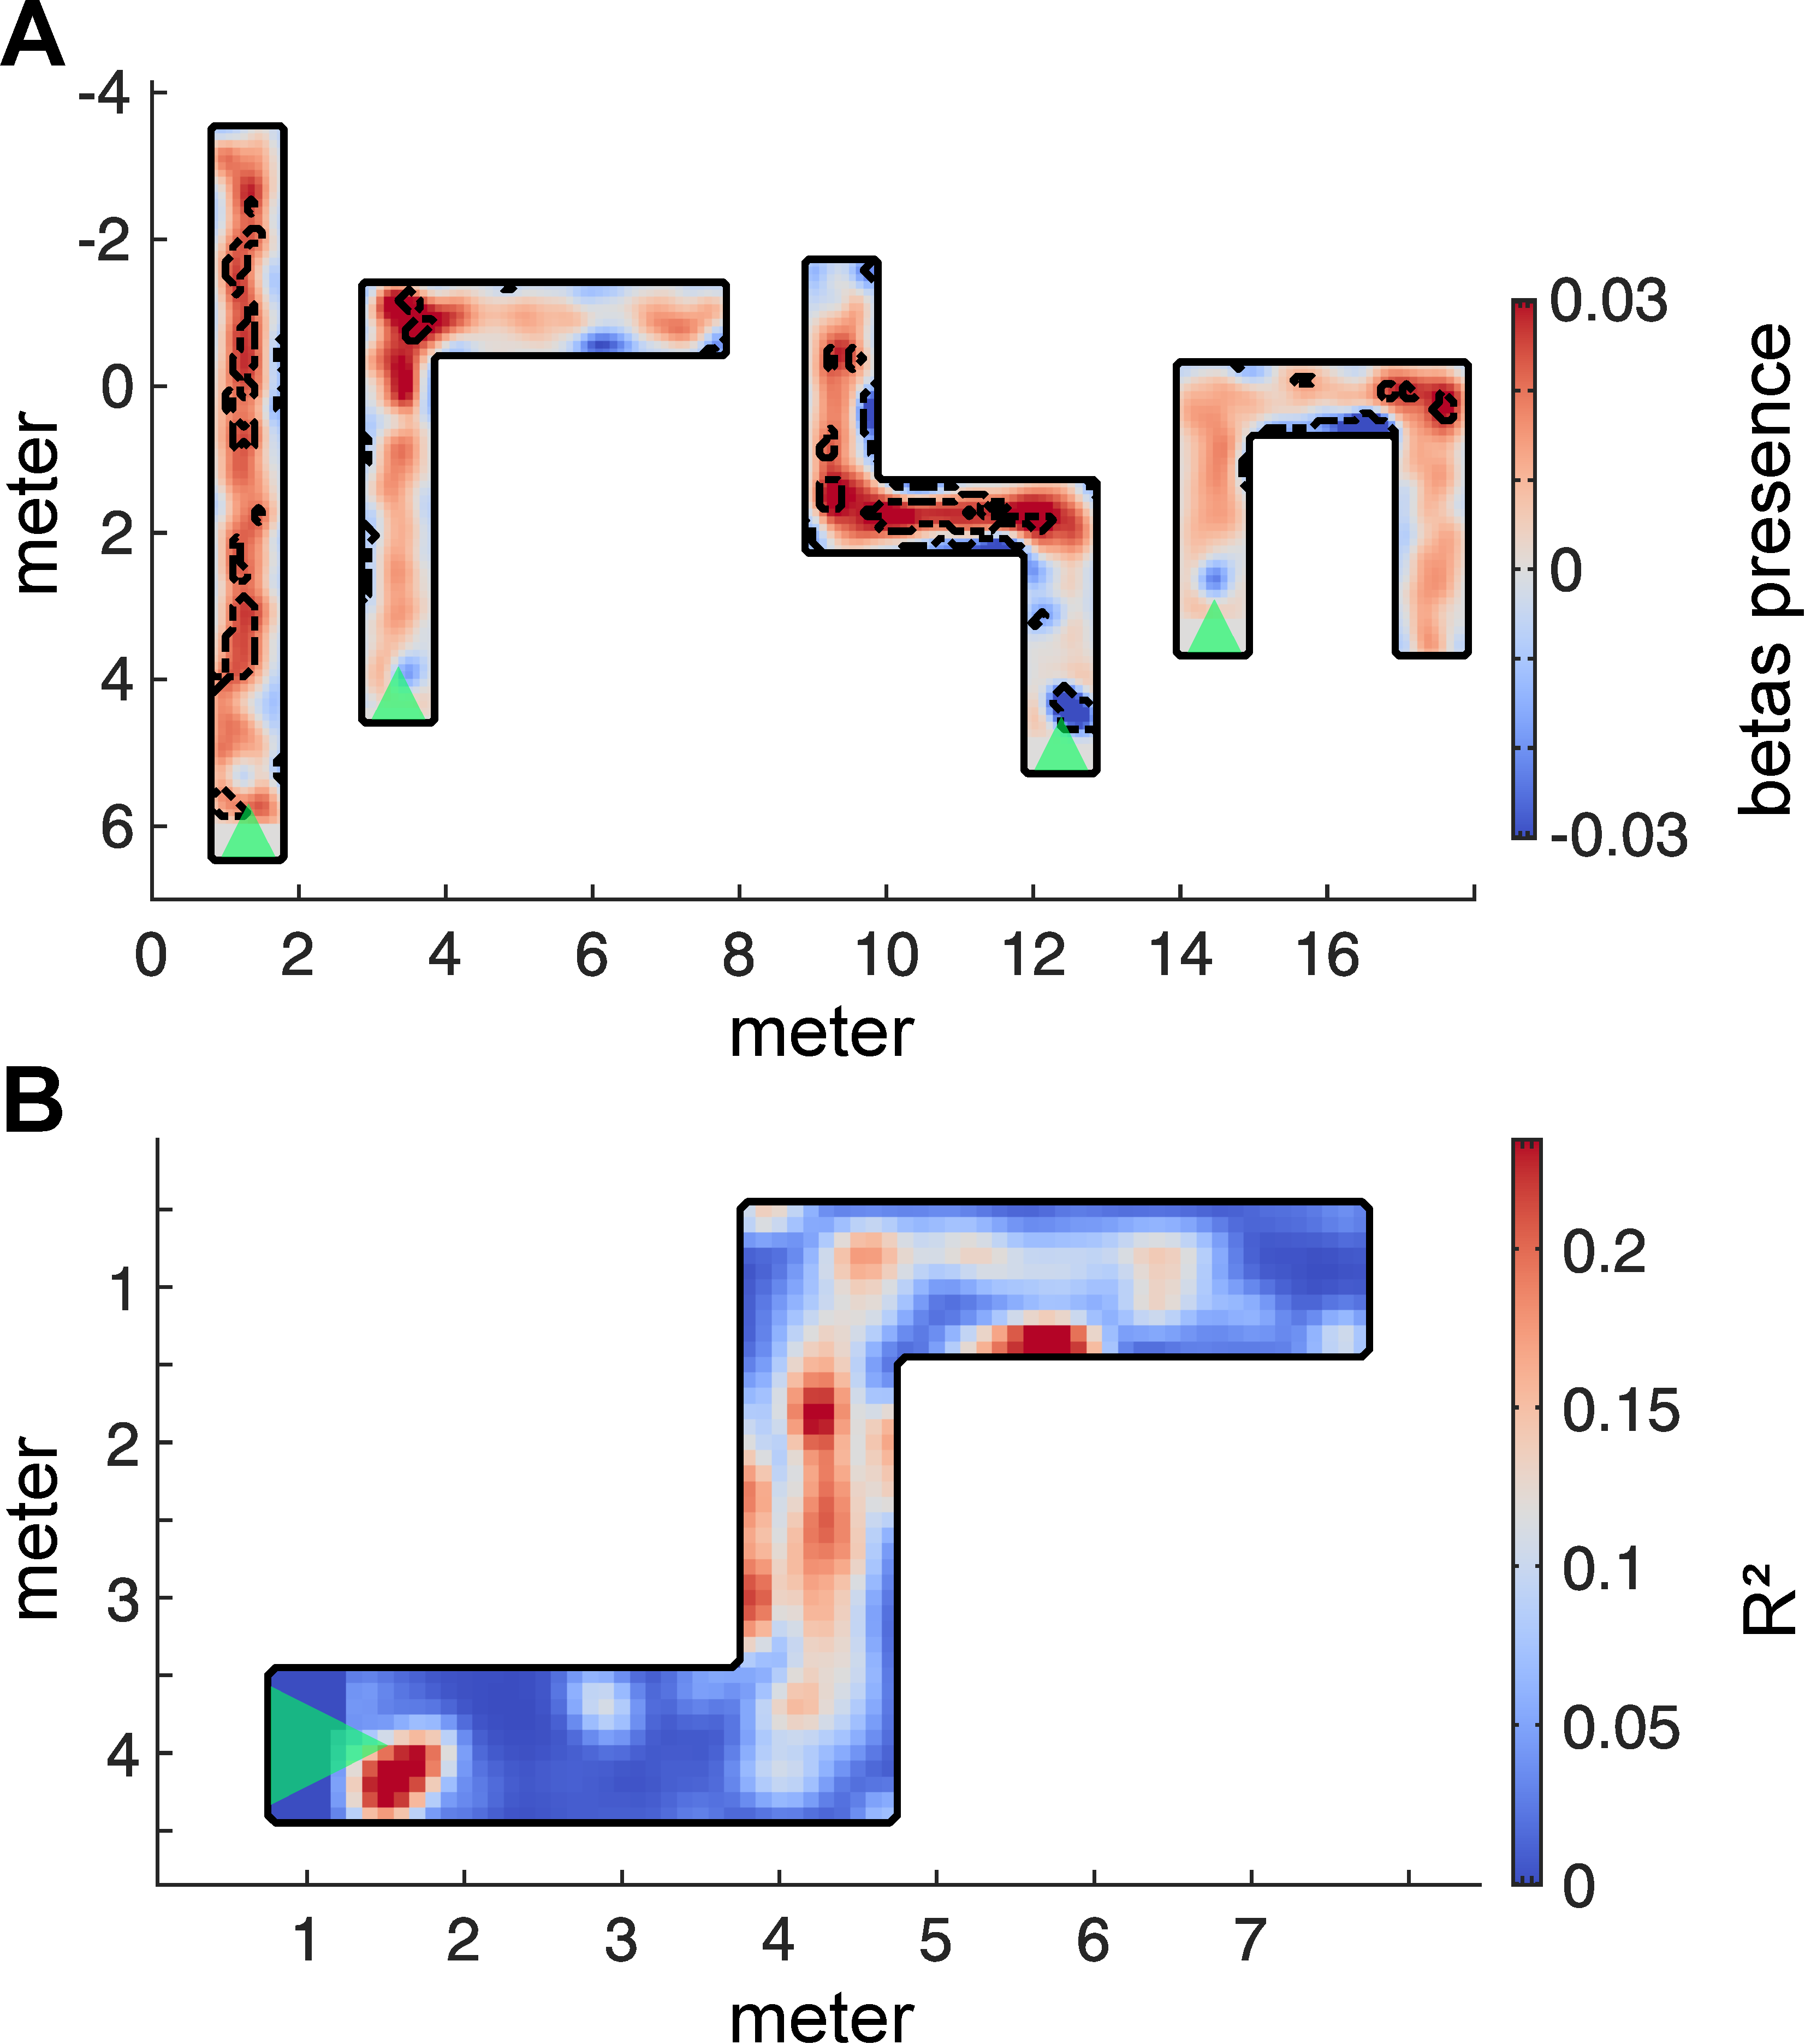
\includegraphics[width=\linewidth]{figures/head_loc_reg2.pdf}
\vspace{6pt}
\caption{Map of the impact of presence on the time spent at every location (betas) in each of the four mazes: `I', `L', `Z', `U'. Green triangles indicate participants starting position. Warmer colors refer to a positive regression estimate. The values can be understood in the sense that for each 1 point increase in reported presence, participants stayed `z' seconds longer at location `xy'. Significant pixels at $p<0.05$ are masked with a dotted line}
\label{presence_head_loc}
\end{figure}

\subsection{Video game experience, biological sex and perspective taking predict presence experience} A step-wise model selection resulted in three remaining predictors, explaining 53,4\% of the variation in experienced presence ($F_{(3,25)}=11.69, p < .001,$ adjusted $R^2=.534$). Participants' predicted presence score was equal to $8.15 - 1.2 (Video Game Experience) + 2.61 (Biological Sex) - 0.02 (PTSOT)$ where biological sex was dummy-coded as 0 = Male, 1 = Female, increasing video game experience was coded with higher scores and decreasing perspective taking ability with higher scores. Video game experience ($t_{(25)}=-4.7, p<.001$), biological  sex ($t_{(25)}=5.6, p<.001$) as well as perspective taking ability ($t_{(25)}=-2.52, p=.02$) were significant predictors of presence. Cross-validation of the three predictor model above yielded a combined average 0.76 mean absolute error. Hence, using video game experience, biological sex as well as perspective taking ability we were able to predict experienced presence with a deviation of $\pm 0.75$ points from the true value on the `IPQ Likert scale'.